\section{Simulation}


\subsection{RAT}
A monte-carlo simulation of particle interactions in the detector is used
for predicting detector observables for events.
The simulation package used is called RAT, it is a Geant4-based simulation that
contains a detector and DAQ simulation in addition to simulation of particle
interactions and photon propagation.


\subsection{Solar Neutrino Fluxes}
\begin{figure}[htbp]
\centering
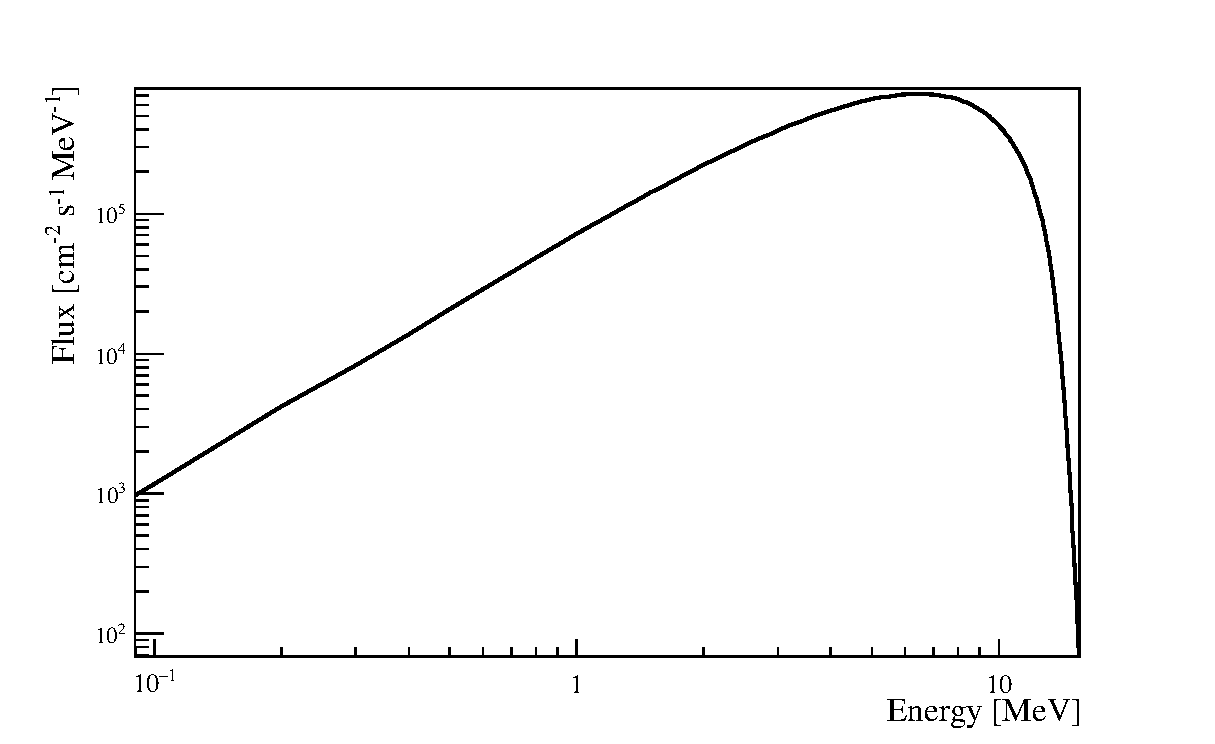
\includegraphics[width=0.75\textwidth]{b8_flux}
\caption[Expected $\ce{^{8}B}$ Flux]{The $\ce{^{8}B}$ neutrino flux
normalized to the solar reaction rate predicted by BS05-0P~\cite{bs05op}}
\label{fig:b8_flux}
\end{figure}
The distribution for the $\ce{^{8}B}$ neutrino energy from Winters~\textit{et. al}~\cite{winterspectrum}
was used, normalized to a nominal flux of $5.69\times10^{6}\mathrm{cm}^{-2}\mathrm{s}^{-1}$,
as predicted by BS05-OP~\cite{bs05op} using the GS98~\cite{gs98} solar
abundances.
This nominal flux normalization is arbitrary because it's the value that is
eventually extracted from data.

\subsection{Solar Neutrino Cross-sections}
The rate of solar neutrino for a given flux follows from the cross-section for
interaction. The only interaction relevant for the SNO+ detector is the
neutrino-electron elastic scattering interaction.
%Neutrino-nuclear interactions occur as well, but they either cannot be identified
%separately from the radioactive backgrounds, or they occur at a very small rate
%compared to the elastic-scattering rate.

The cross-section for the elastic-scattering interaction is take from Bahcall
\textit{et. al}~\cite{escrosssec} which includes radiative corrections to
the cross-section.

\subsection{Survival Probability Simulation}
A simulation of the expected solar survival probability curve for a given
set of mixing parameters was used.
The survival probability is calculated using a
3-flavor adiabatic calculation. The calculation was developed by the
SNO collaboration~/cite{XXX}.
is used to calculate the fraction of the solar neutrino flux that arrives
at Earth and interacts as a $\nu_{e}$ vs the fraction that is $\nu_{\mu}$ or $\nu_{\tau}$.
Solar densities and production distributions from the GS98~\cite{gs98}.

